%--------------------------------------------------------------- %
\documentclass[SPC-MASTER.tex]{subfiles}
\begin{document}
\Large
\section{CUSUM Charts}
\begin{itemize}
\item CUSUM charts, while not as intuitive and simple to operate as Shewhart charts, have been shown to be more efficient in detecting small shifts in the mean of a process. \item In particular, analyzing ARL's for CUSUM control charts shows that they are better than Shewhart control charts when it is desired to detect shifts in the mean that are 2 sigma or less.
\end{itemize}



% http://www.itl.nist.gov/div898/handbook/pmc/section3/pmc323.htm

\begin{figure}[h!]
\centering
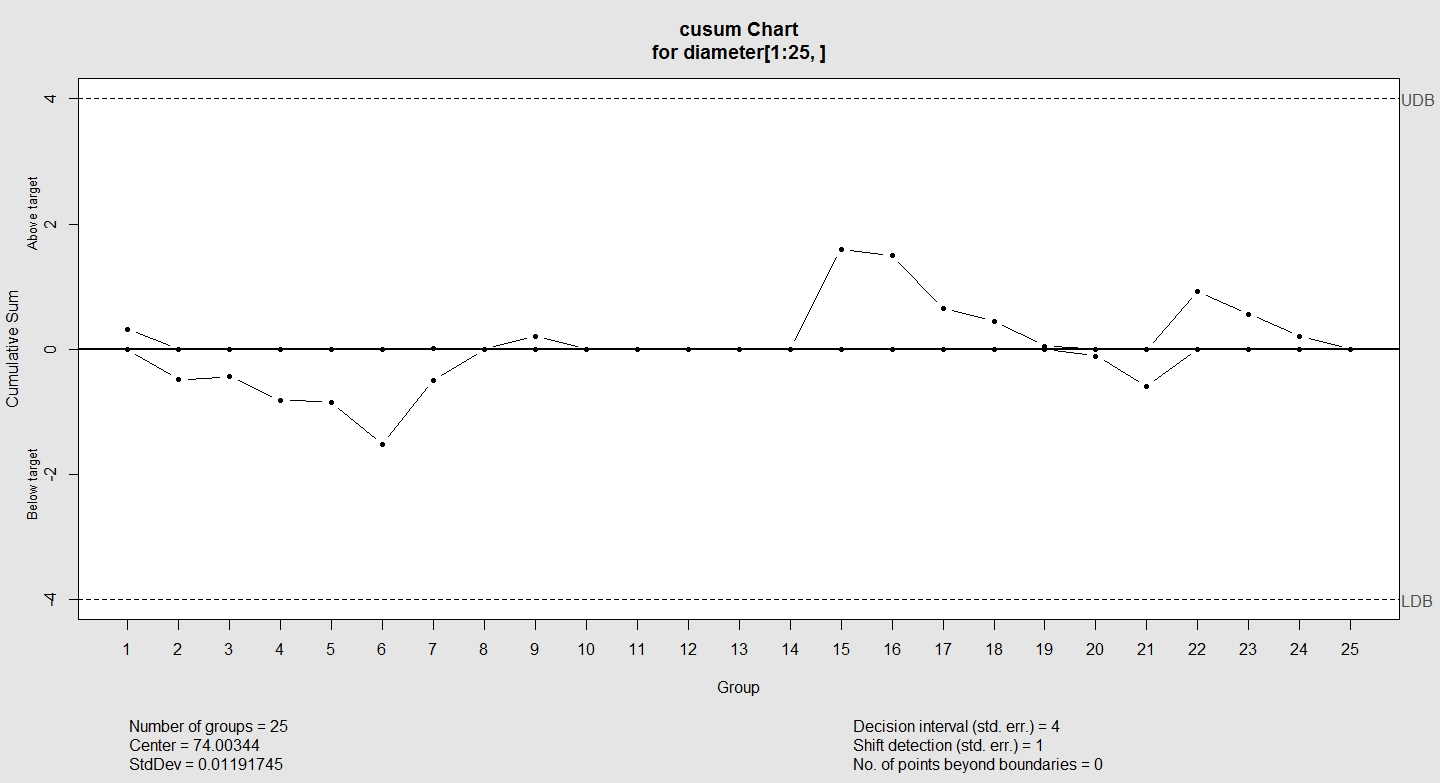
\includegraphics[width=0.7\linewidth]{images/CUSUMorings1}
\caption{}
\label{fig:CUSUMorings1}
\end{figure}

\begin{figure}[h!]
\centering
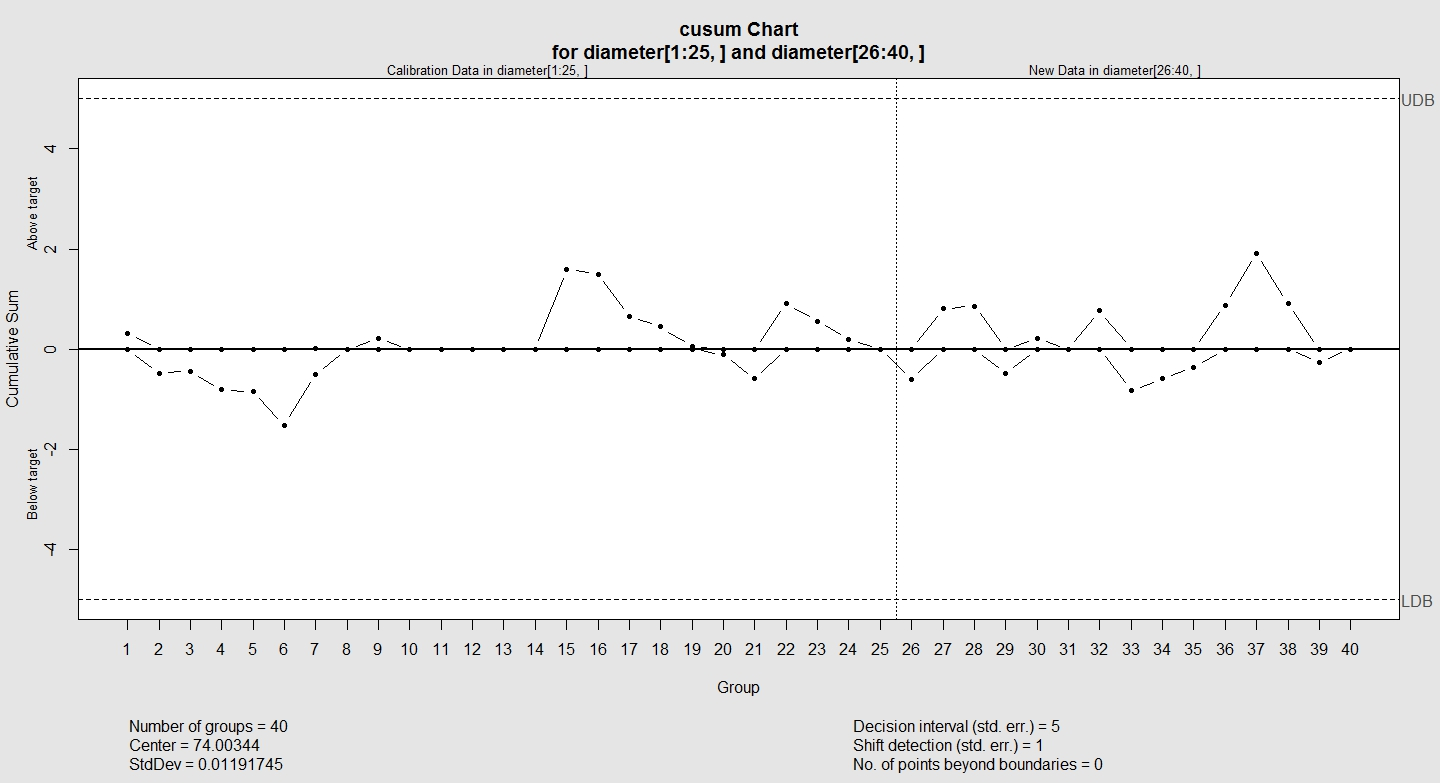
\includegraphics[width=0.7\linewidth]{images/CUSUMorings2}
\caption{}
\label{fig:CUSUMorings2}
\end{figure}


\end{document}